\section{Appendix}

In the following, we describe our previous work that was done towards considering safe reinforcement learning. 
Precisely, we were motivated by the lack of safety guarantees and the use of symbolic reasoning towards incorporating 
safety properties from a verified safe controller (SC) i.e. a declarative language module to compute safe and unsafe states. 
Those safety states are computed during training, thus ensuring that no unsafe states are explored 
by the RL. The general idea was to allow training in the real-world, thus taking away the need for simulation. Our proposed RL+SC architecture is shown in Figure \ref{fig:rlsc}.


\begin{figure}[H]
  \centering
  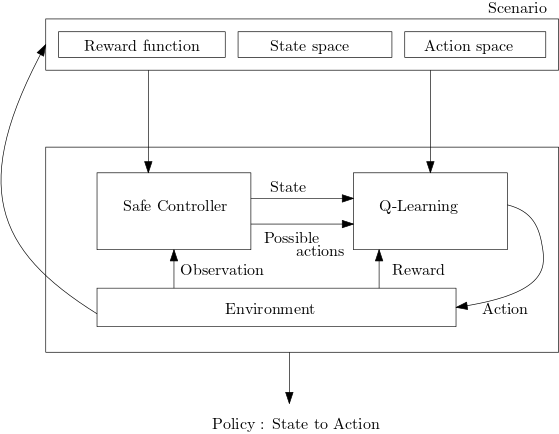
\includegraphics[scale=0.5]{figures/rlsc.png}
  \caption{Overview of the proposed solution}
  \label{fig:rlsc}
\end{figure}

\begin{enumerate}
  \item The environment sends the observation to the SC. 
  \item The SC computes the state from the observation, thus keeping only 
        ground facts that uphold the \emph{Markov Property} (see Definition 9.1). 
  \item The SC also computes the set of possible actions $A$ that ensure that no unsafe states is 
        reached. This is done by searching for possible configurations that follow a (state, action) pair over 
        all possible actions from the action spaces. 
  \item The state and set of possible actions is sent to the RL algorithm, thus only allowing 
        the agent to choose from the set actions. 
  \item Next steps follow from the RL basic routine from Figure \ref{fig:rl}
\end{enumerate}

The implementation can be found in the thesis corresponding github under the rl-implementation folder\footnote{https://github.com/natvern/Thesis}.
For our case study, we chose the vehicle platooning problem. The setting is as follows; two vehicles, one leader and one follower. Their goal is to 
minimize the gap between them while ensuring that they do not crash. 

\medskip

We then present our preliminary results before arguing for the issues with our approach. 

\begin{figure}[H]
  \centering
  \begin{minipage}{.5\textwidth}
    \centering
    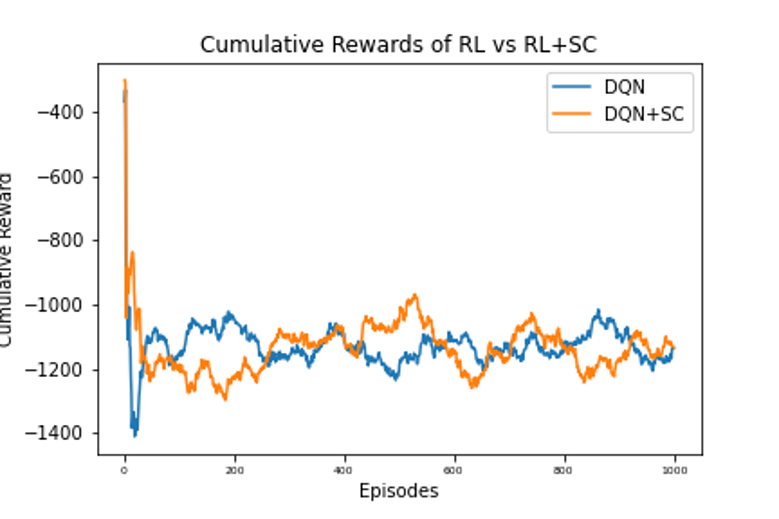
\includegraphics[width=1\linewidth]{figures/appendixopt.png}
    \captionof{figure}{Cumulative Rewards of RL vs. RL+SC}
    \label{fig:optsc}
  \end{minipage}%
  \begin{minipage}{.5\textwidth}
    \centering
    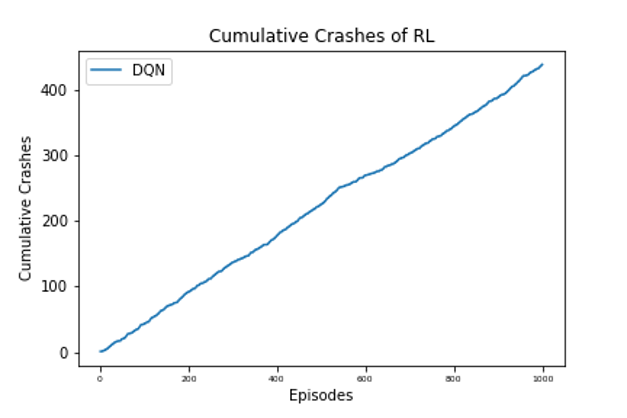
\includegraphics[width=1\linewidth]{figures/appendixcrash.png}
    \captionof{figure}{Cumulative Crashes of RL during Training}
    \label{fig:crashsc}
  \end{minipage}
\end{figure}
  
The graph in Figure \ref{fig:optsc} shows the cumulative rewards of the basic RL implementation without
the safe controller (blue line) vs. the RL+SC implementation (orange line). As evident in the cumulative rewards, all are negative. This is because of our reward function choice 
that only punishes for distances not equal to the desired gap. Thus, learning is not optimal. We can however see that the cumulative rewards of both implementation does not change by a significant 
amount. The graph in Figure \ref{fig:crashsc} shows 
the number of crashes of the basic RL during training. We can easily deduce from the linear graph that the RL without the SC never learns not to crash.


\begin{definition}[Markov Property]
  The next state only depends on the value of the current state. In other words, only the present can affect the future. 
  In terms of our state vector, this means that given $S_t$, I only need the features in $S_t$ to predict $S_{t+1}$.
\end{definition}

\subsection{Issues with the safe RL approach}
\begin{itemize}
  \item The simplicity of our problem setting does not showcase the need for a SC as we only consider two vehicles on an x-axis. 
  \item Though ensuring safety guarantees during training theoretically takes away the need for a simulation, in practice, the uncertainties 
        of the real world cannot be all predicted. This results in a handful of safety properties that might be guaranteed, not enough to allow sensitive cyber-physical systems 
        to be trained using RL in the real world. 
  \item If an oracle existed that was able to predict all uncertainties of the real world, this oracle could then be used to solve the optimization problem 
        deterministically without the need for RL. 
  \item Depending on the SC implementation, safety guarantees can be too strict thus completely destroying optimality. Consider a SC that only allows a car not to move. 
        Though it guarantees that no crashes happen, it is also too strict, thus going against the goal of the agent. 
  
\end{itemize}

\subsection{Reinforcement Learning: Behind the Scenes}
\label{sec:rldetails}
Reinforcement Learning is based on getting sensory input, making a decision, and getting either rewarded or punished for it. 
This method of learning is made possible and effective considering the environment is a \emph{Markov Decision Process}. 
\paragraph{Markov Decision Process (MDP)} Mathematical framework for environments where the outcome of a decision are both affected 
by its stochasticity (e.g. failure in motors) and the decision making of the agent. 
Consider this simple scenario, there exists an agent in a maze whose goal is to escape. The agent at some time $t$ observes that there exists 
walls to his left and to its right, call this state $s_t$, he might then decide to go up, this can either result with probability $p$ into the action actually executing as expected, 
thus moving him a square up to state $s_{t+1}$ or it could fail with probability $1-p$ into going right instead, thus resulting in state  $s'_{t+1}$. 
This is Markov Decision Process. Note specifically that the outcome only depends on what happened a state before. This is similar to \ref{fig:diosim} where worlds 
are instead referred to as states. 
This consideration allows us to define a reward function $R_t(s, s')$ given action $a$. The agent goal is then to maximize its returns 
and come up with a policy that given a state returns the action to take. 
Consequently, we are able to define a value $V$ to a given policy by computing the expected reward from following it. Precisely, 
\begin{equation*}
  V_\pi = E[R \mid s_o=s]
\end{equation*}
There are multiple ways to think about how to maximize this function, those result in different algorithms for Reinforcement Learning. In the following section, 
we present those we've been using. 
\paragraph{Q-Learning}
Q-learning considers the potential reward as the weighted sum of the expected values. It considers the following hyperparameters. 
(1) $\alpha$ the learning rate associated with how much we care about new learning vs. old one, (2) $\gamma$ the discount factor associated with 
the importance of future rewards. At the core of Q-learning is the \emph{Bellman Equation} which results in the following equation. 
\begin{equation*}
  Q_{t'}(s_t, a_t) = Q_{t}(s_t, a_t) + \alpha \times (r_t + \gamma \times max_a Q(s_{t+1}, a) - Q(s_t, a_t) 
\end{equation*}
Precisely, $max_a Q(s_{t+1}, a)$ considers the maximum possible future reward. At its core, the Q-value of a given (state, action) pair 
is dependent on (1) the current value given the learning rate, (2) the reward if we are to take $a$ and finally (3) the maximum 
expected reward that can be obtained in the resulting state. 
\paragraph{Proximal Policy Optimization (PPO)}
We mentioned previous how most of the effort in Reinforcement Learning is fine-tuning the hyperparameters 
and coming up with an effective reward function. PPO strives to find a balance between this fine-tuning and ease of implementation. It ensures so 
by reducing the deviation between $\pi_t$ and $\pi_{t+1}$. 


\subsection{\dio interface} \label{scspecs}
\dio is a logic programming based module that takes the query from the reward function and returns $A$, a judgment that the scenario awaits to update its reward function. The judgment is obscured as it is a choice of the scenario, 
independent of the \dio implementation. In the following, we will define $A$ by its behavior, rather than its type. To do so, we will walk through the routine in the diagram of Figure \ref{fig:diospecs}.
Note that \dio follows a certain interface which we describe in the procedure below.

\begin{figure}[H]
  \centering
  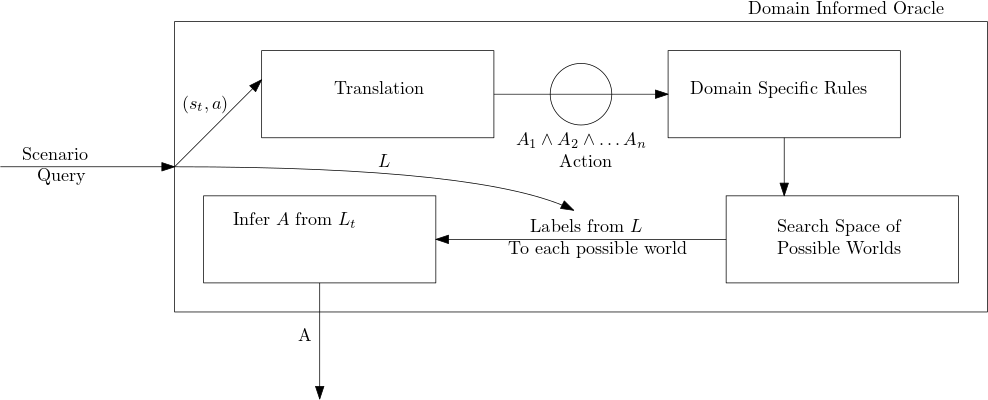
\includegraphics[scale=0.46]{figures/diospecs.png}
  \caption{Domain Informed Oracle routine}
  \label{fig:diospecs}
\end{figure}

\begin{enumerate}
  \item The scenario queries \dio. It sends $(s_t, a)$, the state at time $t$ and the action. It also sends $L : s \rightarrow t$ where $t$ is a sum of types: 
        $t \equiv t_1 + t_2 .. + t_n$. For instance, consider our previous example of the chess game and let the scenario define good openings as "desirable" and random openings as 
        "undesirable". Thus $t \equiv d + ud$ where $d$ is equivalent to desirable and $ud$ to undesirable. 
  \item The first step of \dio is a translation $T : \mathbb{R}^n
  \rightarrow \omicron_1 \times \omicron_2 \times ... \omicron_n$ that takes in the state
  vector $s_t$ and returns a conjunction of propositions $P = A_1 \wedge
  A_2 \wedge ... \wedge A_n$. This is our set of ground facts.
  \item P is passed alongside the action to the domain specific rules defined in \dio. 
  \item Using step semantics, \dio generates possible worlds up to a given time $t'$. Note that given the stochasticity of the environment, there is no certainty on
        whether the worlds expected by \dio will necessarily happen. Consider Figure \ref{fig:diosim}.
  \item Those possible worlds, equivalent to states, can be
  transformed using $L$ to $t$. This is done in a declarative tool, problog in our case. In practice, t
  this labeling takes in the ground facts and generates possible predicates. 
  \item At the last step, \dio ends up with a set $S$ of $t$ that defines the labels of all the possible worlds.
  \item The last step is left as an inference depending on how the the judgment for deciding a final $J$ judgment from $S$ 
        is formulated. For instance, we can consider a rule where if most of the possible worlds are undesirable, then let $J$ be undesirable.
        This judgment can only be a numerical value as we've done in our gridworld example. Precisely, $J$ is the sum of the weighted probabilities of our system at the next 
        timestep.
  \item Finally, $J$ is passed to the scenario. Note then that $J : t$. 
\end{enumerate}

\begin{figure}[H]
  \centering
  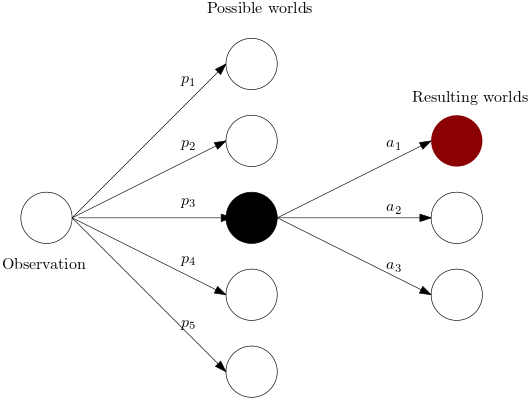
\includegraphics[scale=0.5]{figures/scworlds.png}
  \caption{Game Tree Simulation by \dio}
  \label{fig:diosim}
\end{figure}

Observe how this does not guarantee that the reward function will be informed in a meaningful way.
To that end, we need to consider (1) what are the specifications of a 'good' reward function, (2) what conditions should be set 
on the domain specific rules and $L$ provided by the scenario, (3) how to define a systematic way for the scenario to use 
this information. Those considerations are left for future
investigations. However, note that those problems are existing problems in defining a reward function 
without \dio but made easier to investigate with \dio. This is made possible because the problem 
is not that of writing the reward function given a state vector, rather how to write a reward function given 
$A$. For instance, in our experiments, we label states as either desirable, undesirable or fatal and associate 
the corresponding numerical values $(1,-0.5, -1)$, intuitively. Such a basic labeling gave us good results without 
going through the trial-and-error process that is present in RL. 
